\documentclass[dvips]{beamer}
\usetheme{Madrid}
\usepackage{pgfpages}
\usepackage[usenames,dvipsnames]{pstricks}
\usepackage{amsmath,amssymb,amsthm,amscd}
\usepackage{graphicx}
\usepackage{verbatim}



\mode<presentation>

%Commands used in this document.
\newcommand{\ket}[1]{\left| #1 \right>} % for Dirac bras
\newcommand{\bra}[1]{\left< #1 \right|} % for Dirac kets
\newcommand{\braket}[2]{\left< #1 \vphantom{#2} \right|
 \left. #2 \vphantom{#1} \right>} % for Dirac brackets
\newcommand{\matrixel}[3]{\left< #1 \vphantom{#2#3} \right|
 #2 \left| #3 \vphantom{#1#2} \right>} % for Dirac matrix elements


%Commands used in this document for pstricks pictures.
\def\Hbox(#1){\rput*(#1){\psframebox[boxsep=false,linewidth=1pt]{\small H}}}
\def\Spos{\small$\frac{1}{\sqrt{2^n}}\Sigma_{i=0}^{2^n-1}\left|i\right>$}
\def\Oout{\small$\left|t \oplus{M_{f}}\right>$}
\def\ketx(#1){\small$\left|#1\right>$}
\def\Hi{1}\def\Hii{2}\def\Hiii{5.25}

%definitions from Prof. Das Gupta slides
\definecolor{Maroon}{rgb}{.5,.1,.25}% Used for Trinity University
\definecolor{dgreyblue}{rgb}{0.26,0.3,0.46}             %89.25 102 158.10
\newcommand{\grey}[1]{{\textcolor{dgreyblue}{#1}}}
\newcommand{\truered}[1]{{\textcolor{red}{#1}}}

% *********************** frequently used math symbols from AMS *******
\newcommand{\norm}[1]{\left\Vert#1\right\Vert}
\newcommand{\abs}[1]{\left\vert#1\right\vert}
\newcommand{\set}[1]{\left\{#1\right\}}
\newcommand{\M}{\mathsf{M}}
\newcommand{\opt}{\mathsf{OPT}}
\newcommand{\NP}{\mathsf{NP}}
\newcommand{\apx}{\mathsf{APX}}
\newcommand{\TMIS}{{\bf 3-$\pmb{\mathsf{MIS}}$}}
\newcommand{\dhigh}{{\delta_{h}}}
\newcommand{\dlow}{{\delta_{\ell}}}
\newcommand{\dlowsq}{{\delta^2_{{\ell}}}}
\newcommand{\dhighsq}{{\delta^2_{h}}}
\newcommand{\R}{\mathbb{R}}
\newcommand{\x}{\mathbf{x}}

\begin{document}
\title[Short Title]{Long Title}
\title[GSoC 2012 Sympy]{Google Summer of Code 2012 - Sympy}
\author[Guru Devanla] {Guru Devanla \\ Mentor: Dr. Brian Granger, Physics Professor, Cal State}

\institute[UIC]{\bf%
   {
   Department of Computer Science \\
   University of Illinois at Chicago \\
   Chicago, IL 60607, USA} \\
   {\em gdevan2@cs.uic.edu} \\
}

\date[GSOC Meetup]{\today}

\begin{frame}
\titlepage
\end{frame}


% \AtBeginSection[]
% {
%   \begin{frame}<beamer>
%   \frametitle{Outline}
%   {\bf \tableofcontents[currentsection, currentsubsection]}
%   \end{frame}
% }

% \AtBeginSubsection[]
% {
%   \begin{frame}<beamer>
%   \frametitle{Outline}
%   \tableofcontents[currentsection, currentsubsection]
%   \end{frame}
%}

\frame{\tableofcontents}

\section{Sympy}
\subsection{What is Sympy?}

\begin{frame}
\frametitle{What is Sympy}
\begin{itemize}
\item A Python library for \emph{symbolic mathematics}
\item Has a goal of becoming a full featured \emph{Computer Algebra System}
\item Written entirely in Python and does not require external libraries
\end{itemize}
\vspace*{0.5in}
\tiny{[1] : http://sympy.org/en/index.html}

\end{frame}

\subsection{Sympy - Features}
\begin{frame}
\frametitle{Sympy 0.7.1 - Features}

\begin{itemize}
\item Core Capabilities
\pause
\item Other Modules
  \begin{itemize}
     \item Polynomials
     \item Calculus
     \item Solving Equations
     \item Discrete Math
     \item Matrices
     \item ....
     \item Physics
        \begin{itemize}
              \item Mechanics
              \item Quantum : Quantum Mechanics, Qubits, Quantum Gates etc.
              \item ( GSOC 2012 : Density Operator)
        \end{itemize}
  \end{itemize}
\pause
\item Printing
  \begin{itemize}
    \item \LaTeX, MathML etc
  \end{itemize}
 \end{itemize}
\end{frame}


\subsection{Examples}
\begin{frame}
\frametitle{Examples}
\includegraphics[height=2in,width=3in]{ex1.ps}\newline
\tiny{source: http://sympy.org}
\end{frame}

\begin{frame}
\frametitle{Examples}
\includegraphics[height=2in,width=3in]{ex2.ps}\newline
\tiny{source: http://sympy.org}
\end{frame}


\begin{frame}
\frametitle{Examples}
\includegraphics[height=2in,width=3in]{ex3.ps}\newline
\tiny{source: http://sympy.org}
\end{frame}

\begin{frame}
\frametitle{Examples}
\includegraphics[height=2in,width=2in]{ex4.ps}\newline
\tiny{source: http://sympy.org}
\end{frame}

\begin{frame}
\frametitle{Examples}
\includegraphics[height=2in,width=2in]{ex5.ps}\newline
\tiny{source: http://sympy.org}
\end{frame}


\section{Sympy - Quantum Module}
\subsection { States as Vectors }
\begin{frame}
\frametitle{Sympy - Quantum Module}

Informally , in quantum mechanics, \emph{states} in a closed system are
represented as linear combination of a set of basis vectors,
\newline
\[State: \left[
\frac{1}{\sqrt{2}} \left( \begin{matrix} 1 \\ 0 \end{matrix} \right)
+ \frac{1}{\sqrt{2}}
\left( \begin{matrix}  0 \\ 1 \end{matrix} \right)
\right]\]

where \newline

${(\frac{1}{\sqrt{2}})}^2 = 0.5$ gives the probability of observing either state.


\end{frame}


\begin{frame}
\frametitle{Mixed States}

Say we have 2 states, given by

\[
State_1 : \frac{1}{\sqrt{2}} \left( \begin{smallmatrix} 1 \\ 0 \end{smallmatrix} \right)
+ \frac{1}{\sqrt{2}}
\left( \begin{smallmatrix}  0 \\ 1 \end{smallmatrix} \right)
\]

with $Pr(State_1)=\frac{1}{3}$

\[ State_2:
\frac{1}{\sqrt{2}} \left( \begin{smallmatrix} 1 \\ 0 \end{smallmatrix} \right)
- \frac{1}{\sqrt{2}}
\left( \begin{smallmatrix}  0 \\ 1 \end{smallmatrix} \right)
\]
with $\Pr(State_2) = \frac{2}{3}$
\newline\newline\newline
\pause
\small{Represented as} \[\left( (state_1, p_1), (state_2,p_2)....(state_n,p_n) \right)\]

This representation becomes quite cumbersome.

\end{frame}

\subsection {Density Matrices(Operators)}
\begin{frame}
\frametitle{Density Matrices}


Density Matrix($\rho$) given by
\newline
\texttt{sum of outer products of each of these states}

\[\rho =  \sum_{i=1}^{n} p_i(state_i) .  (p_i(state_i))^* \]

\pause
This gives us a nice matrix. \newline
\begin{itemize}
\item Helps in representation
\item Used to evaluate various properties about systems in mixed states
\end{itemize}


\end{frame}

\subsection {  Goals - Density Operator Implementation }
\begin{frame}
\frametitle{GSoC 2012 - Project Goals }

\begin{itemize}
\item Methods to declare density matrices
\item Extend operators for time dependent states
\item Way to use these objects in equations representing quantum circuits
\item Integrate with current eval() functions to work with other quantum
  expressions
\end{itemize}

\end{frame}

\subsection {  Tools / Workflow }
\begin{frame}
\frametitle{Tools/Workflow}
\begin{itemize}
\item Python 2.7
\item IPython as interactive python shell
\item Emacs powered with python-mode, pymacs and pyrope
\item git and github
\end{itemize}

\end{frame}


\subsection{ More resources }
\begin{frame}
\frametitle{live.sympy.org}
\includegraphics[height=3in,width=4in]{ex6.ps}
\end{frame}


\end{document}

